\documentclass[11pt]{article}

\usepackage{outlines}
\usepackage{graphicx}
\usepackage[T1]{fontenc}
\usepackage{subcaption}
\usepackage[margin=1in]{geometry}

\usepackage{geometry}
\usepackage[square,sort,comma,numbers,super]{natbib}
\usepackage{pdflscape}
\usepackage{hyperref}
\usepackage{afterpage}
\usepackage{listings}

\graphicspath{ {./images/} }

\setlength{\parindent}{0pt}

% pt = project title; shorthand
\newcommand{\pt}{Multi-User Poker Game}
\newcommand{\pn}{Rekop}

\title{Interim Report: \pt}
\author{James Scully}



\begin{document}

{\fontfamily{cmss}\selectfont}



\newcommand{\cardheight}{6em}

\newcommand{\tenclubs}{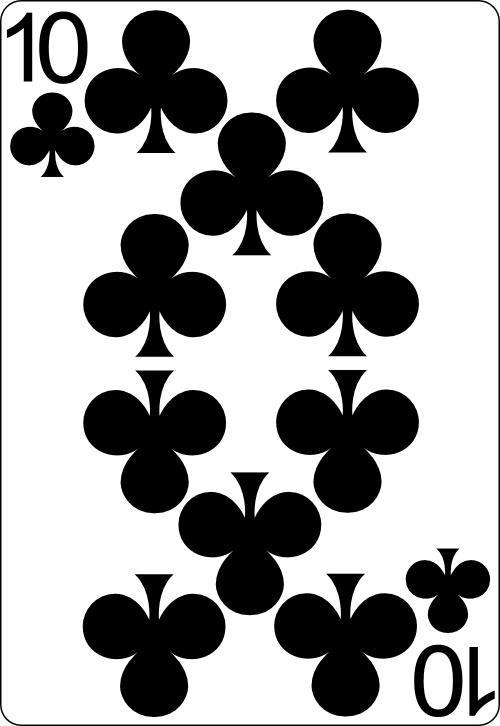
\includegraphics[height=\cardheight]{cards/10_of_clubs.png}}
\newcommand{\tendiamonds}{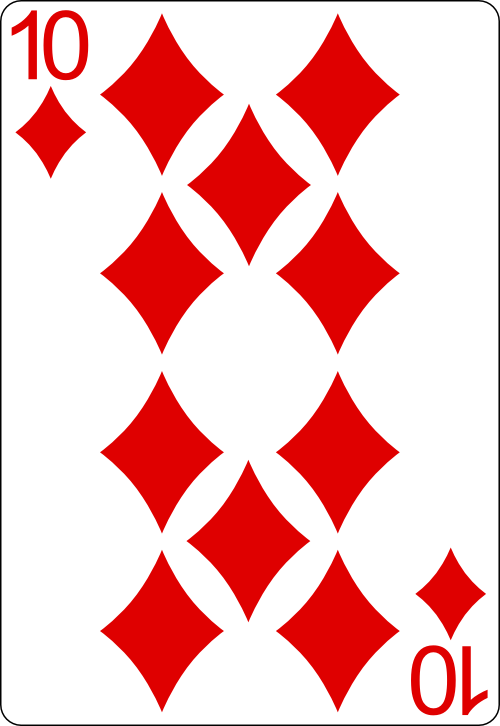
\includegraphics[height=\cardheight]{cards/10_of_diamonds.png}}
\newcommand{\tenhearts}{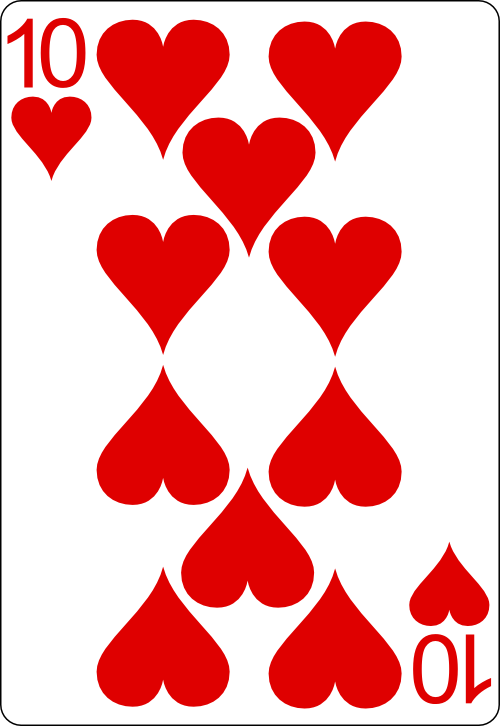
\includegraphics[height=\cardheight]{cards/10_of_hearts.png}}
\newcommand{\tenspades}{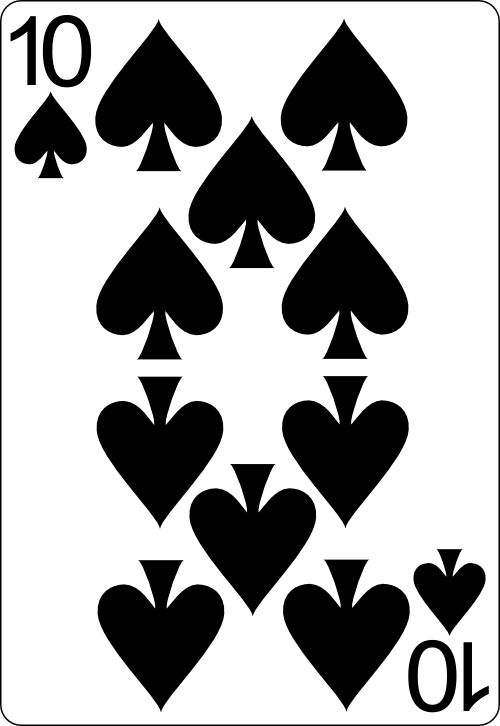
\includegraphics[height=\cardheight]{cards/10_of_spades.png}}
\newcommand{\twoclubs}{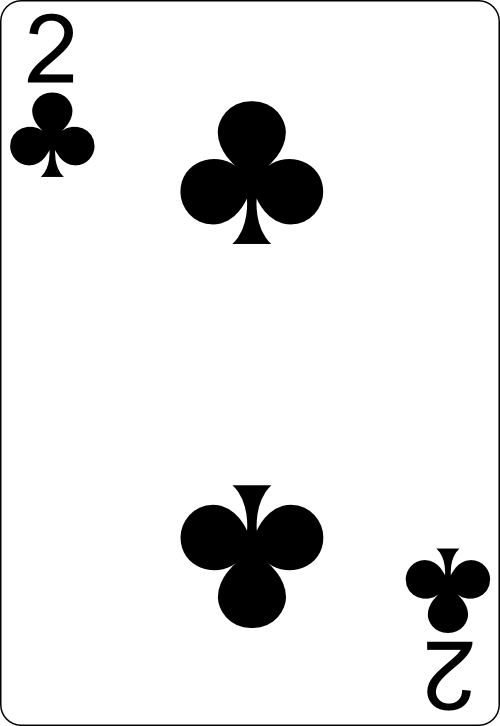
\includegraphics[height=\cardheight]{cards/2_of_clubs.png}}
\newcommand{\twodiamonds}{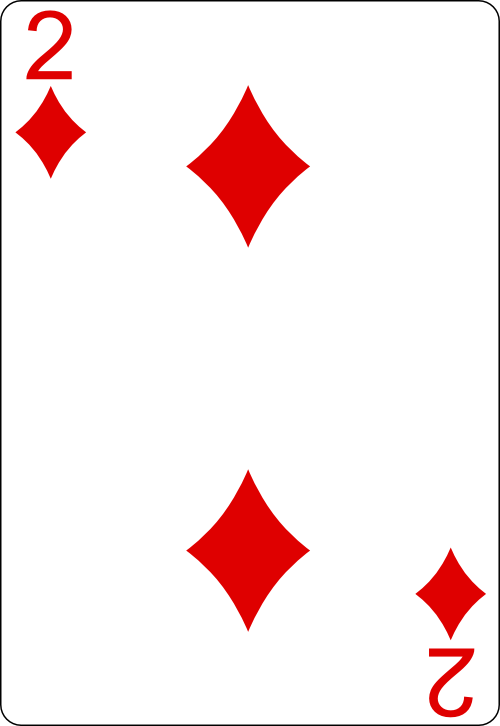
\includegraphics[height=\cardheight]{cards/2_of_diamonds.png}}
\newcommand{\twohearts}{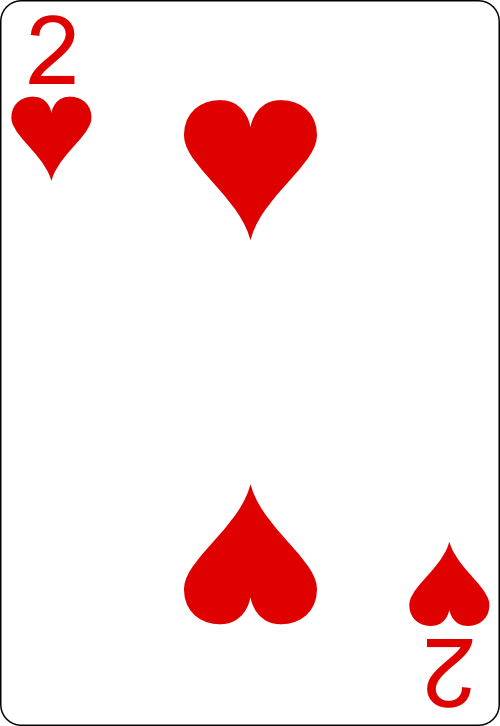
\includegraphics[height=\cardheight]{cards/2_of_hearts.png}}
\newcommand{\twospades}{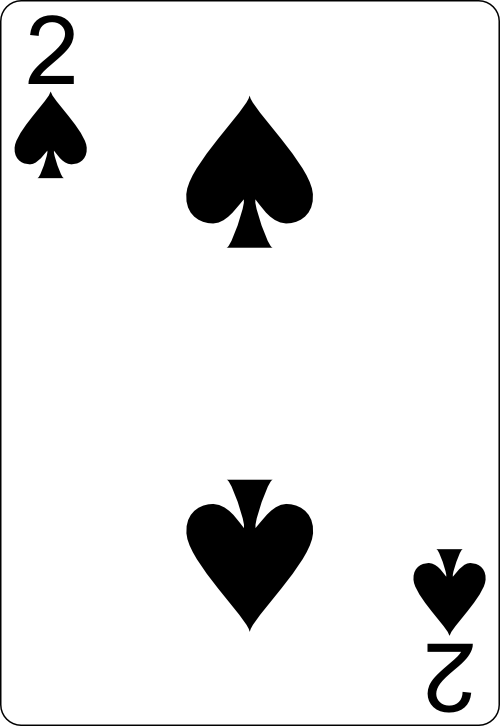
\includegraphics[height=\cardheight]{cards/2_of_spades.png}}
\newcommand{\threeclubs}{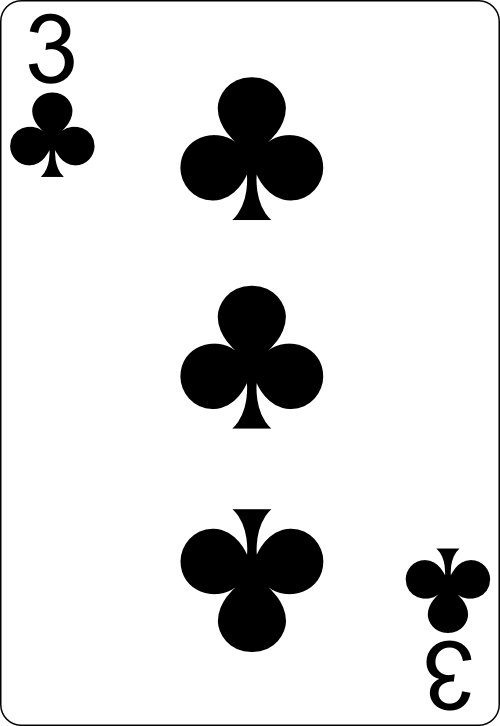
\includegraphics[height=\cardheight]{cards/3_of_clubs.png}}
\newcommand{\threediamonds}{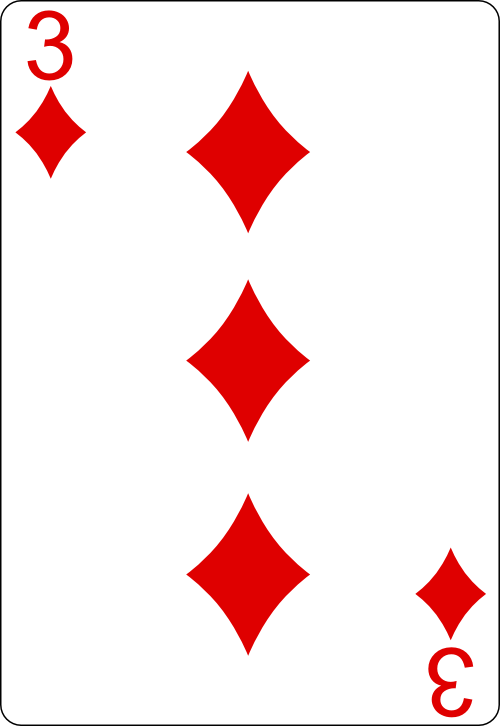
\includegraphics[height=\cardheight]{cards/3_of_diamonds.png}}
\newcommand{\threehearts}{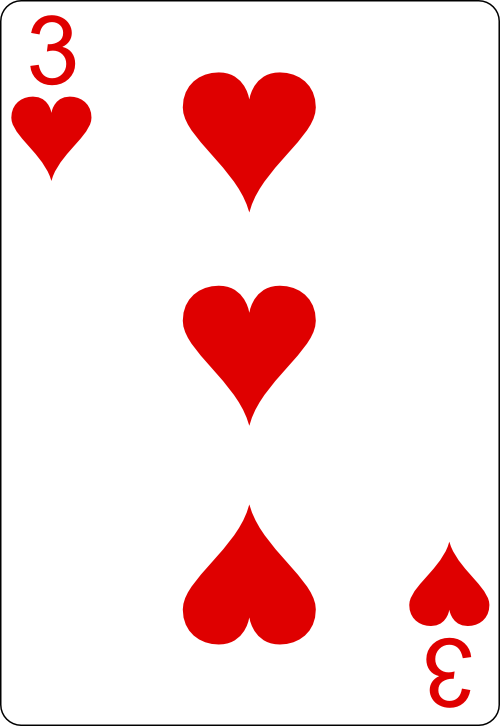
\includegraphics[height=\cardheight]{cards/3_of_hearts.png}}
\newcommand{\threespades}{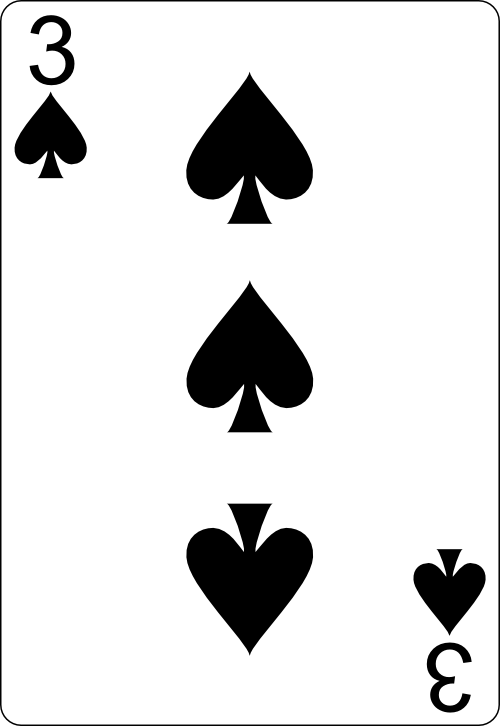
\includegraphics[height=\cardheight]{cards/3_of_spades.png}}
\newcommand{\fourclubs}{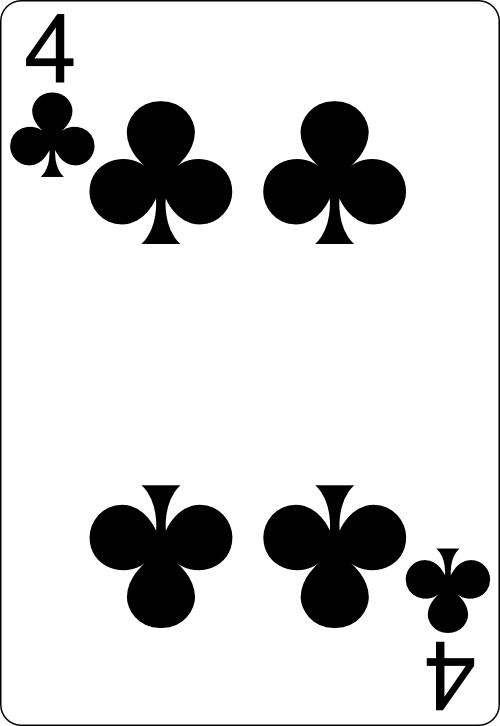
\includegraphics[height=\cardheight]{cards/4_of_clubs.png}}
\newcommand{\fourdiamonds}{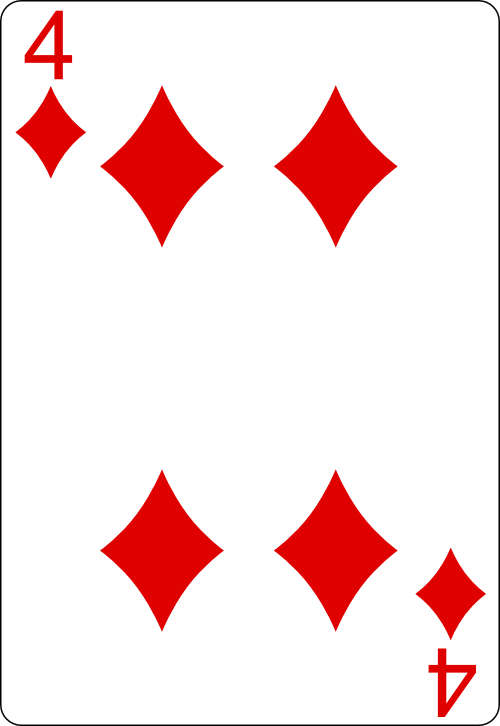
\includegraphics[height=\cardheight]{cards/4_of_diamonds.png}}
\newcommand{\fourhearts}{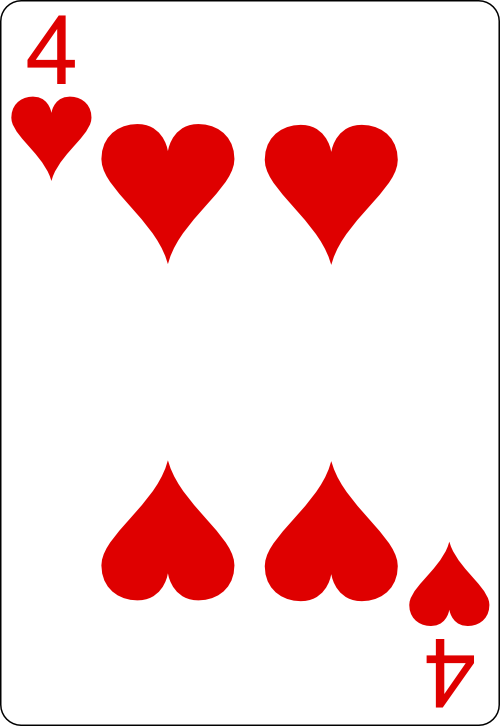
\includegraphics[height=\cardheight]{cards/4_of_hearts.png}}
\newcommand{\fourspades}{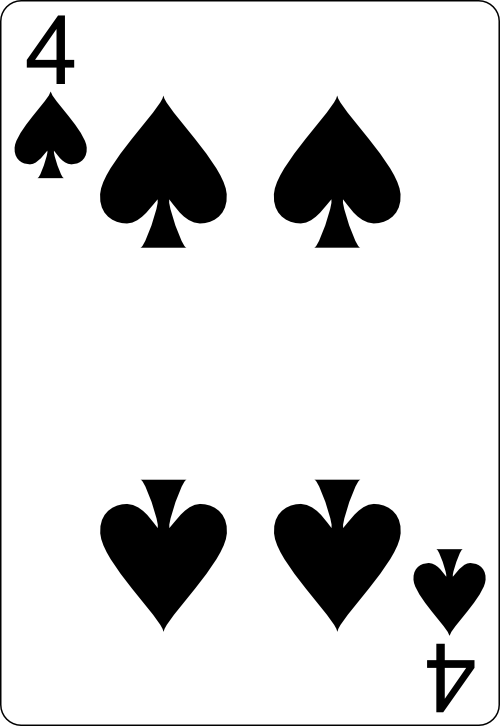
\includegraphics[height=\cardheight]{cards/4_of_spades.png}}
\newcommand{\fiveclubs}{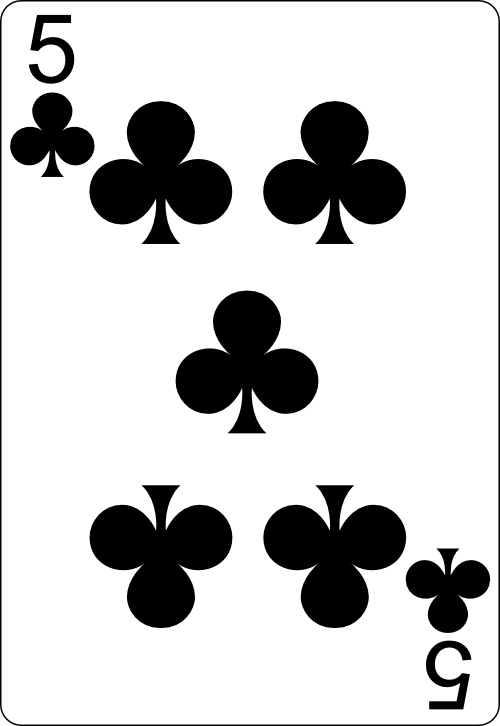
\includegraphics[height=\cardheight]{cards/5_of_clubs.png}}
\newcommand{\fivediamonds}{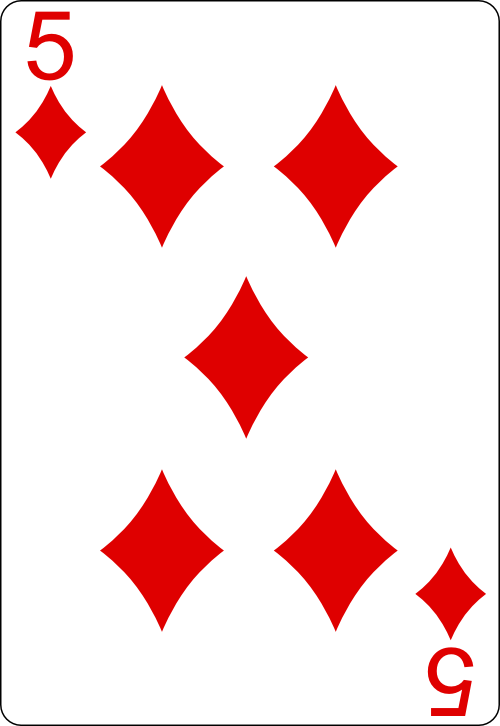
\includegraphics[height=\cardheight]{cards/5_of_diamonds.png}}
\newcommand{\fivehearts}{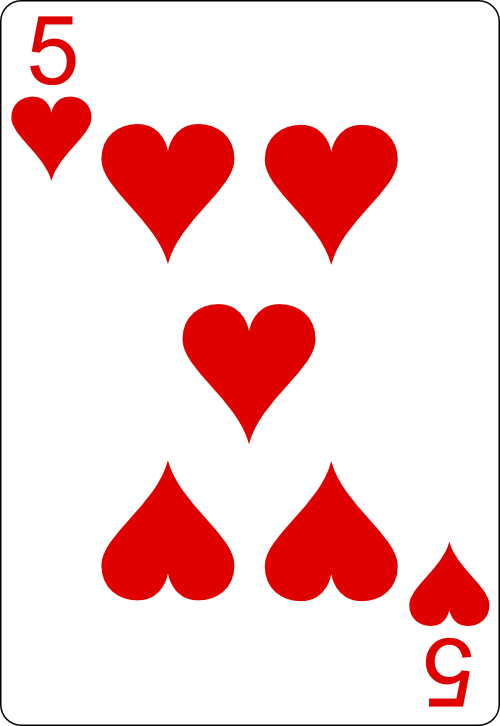
\includegraphics[height=\cardheight]{cards/5_of_hearts.png}}
\newcommand{\fivespades}{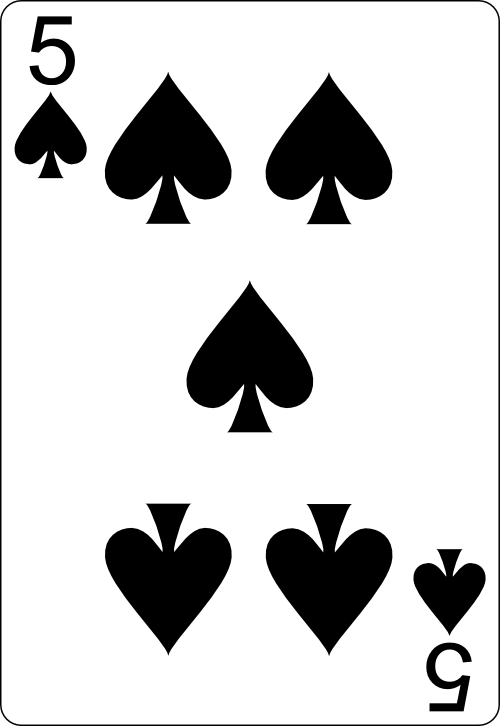
\includegraphics[height=\cardheight]{cards/5_of_spades.png}}
\newcommand{\sixclubs}{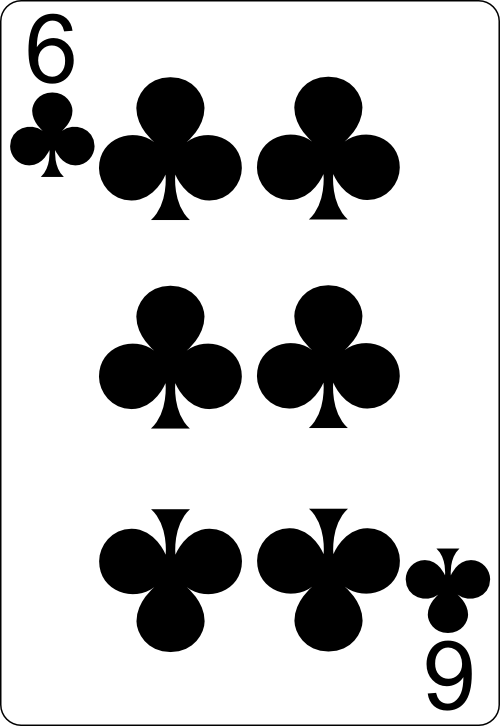
\includegraphics[height=\cardheight]{cards/6_of_clubs.png}}
\newcommand{\sixdiamonds}{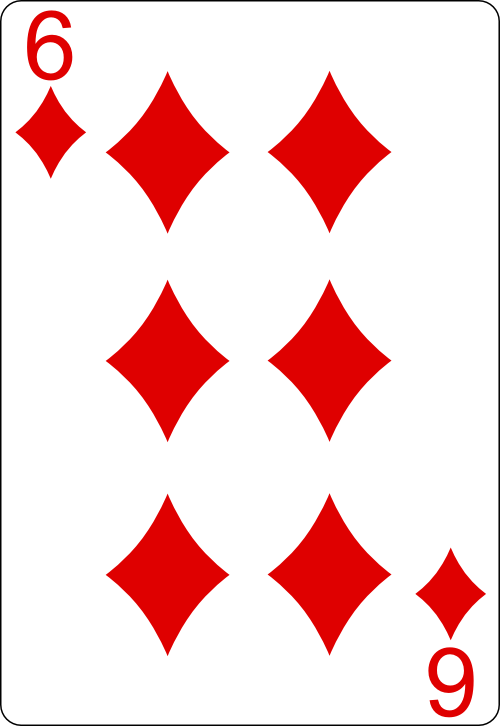
\includegraphics[height=\cardheight]{cards/6_of_diamonds.png}}
\newcommand{\sixhearts}{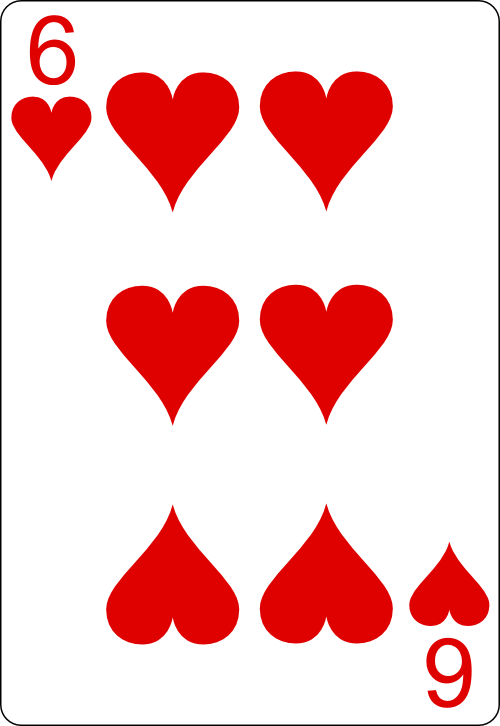
\includegraphics[height=\cardheight]{cards/6_of_hearts.png}}
\newcommand{\sixspades}{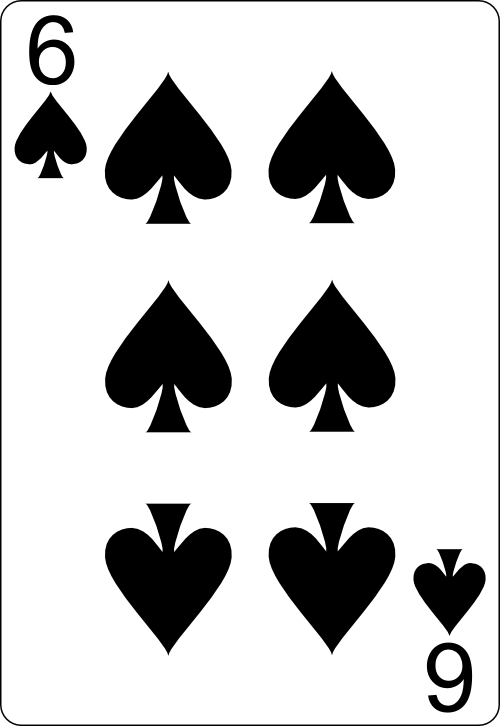
\includegraphics[height=\cardheight]{cards/6_of_spades.png}}
\newcommand{\sevenclubs}{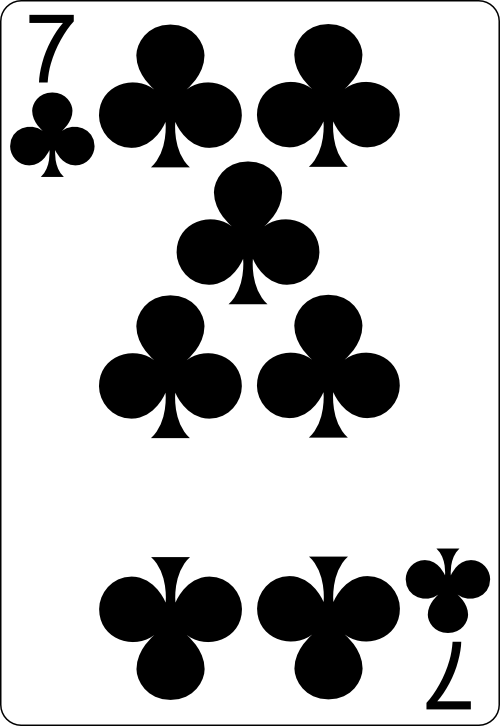
\includegraphics[height=\cardheight]{cards/7_of_clubs.png}}
\newcommand{\sevendiamonds}{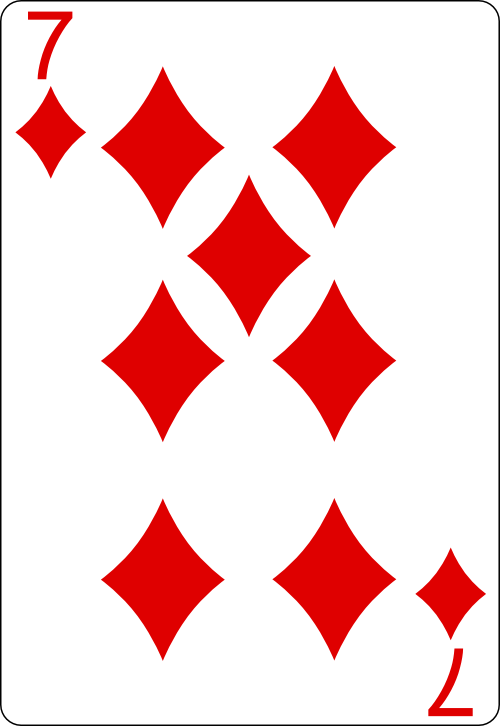
\includegraphics[height=\cardheight]{cards/7_of_diamonds.png}}
\newcommand{\sevenhearts}{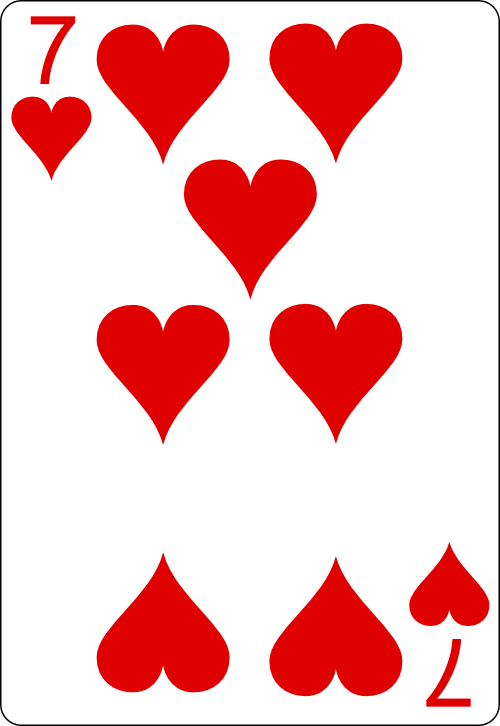
\includegraphics[height=\cardheight]{cards/7_of_hearts.png}}
\newcommand{\sevenspades}{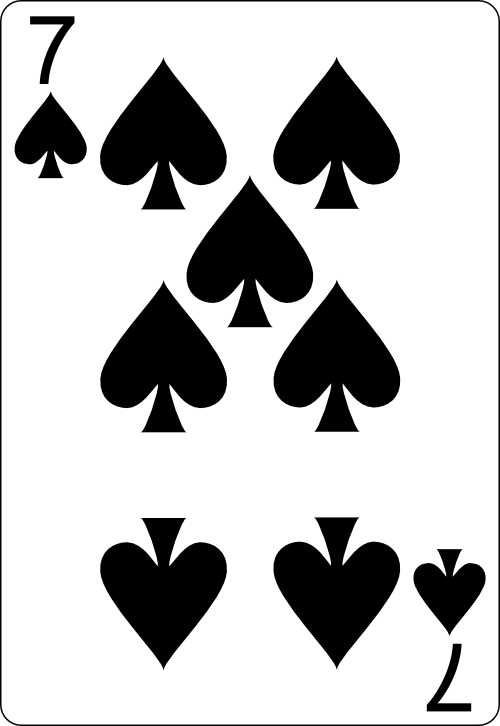
\includegraphics[height=\cardheight]{cards/7_of_spades.png}}
\newcommand{\eightclubs}{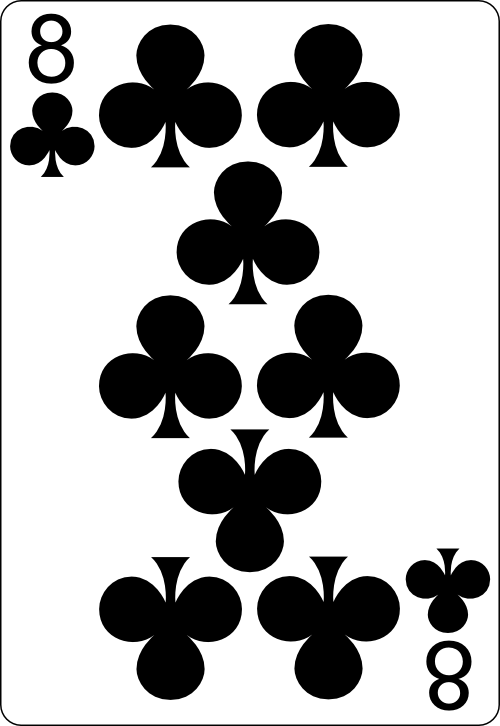
\includegraphics[height=\cardheight]{cards/8_of_clubs.png}}
\newcommand{\eightdiamonds}{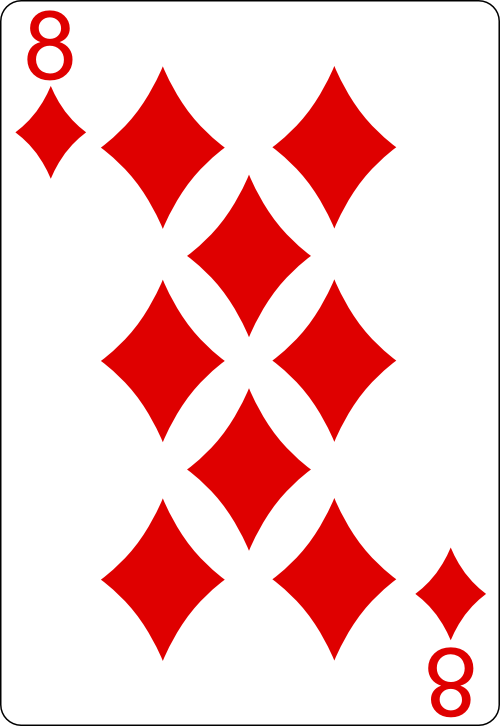
\includegraphics[height=\cardheight]{cards/8_of_diamonds.png}}
\newcommand{\eighthearts}{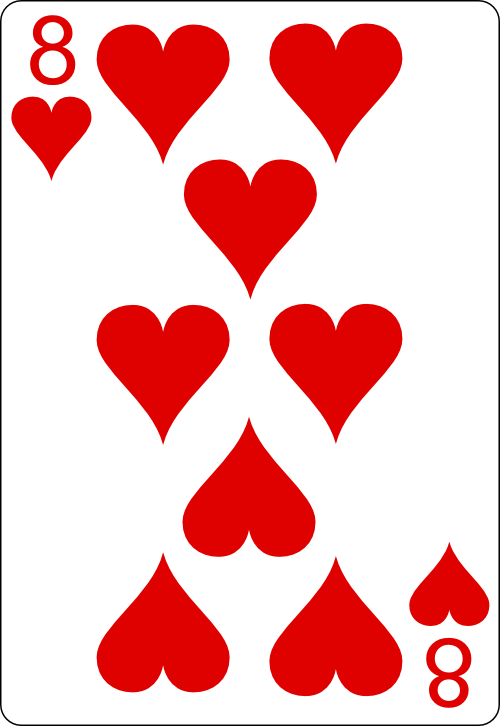
\includegraphics[height=\cardheight]{cards/8_of_hearts.png}}
\newcommand{\eightspades}{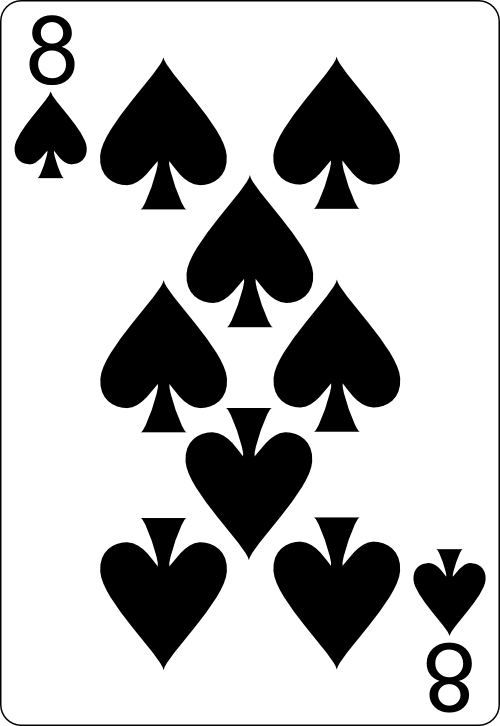
\includegraphics[height=\cardheight]{cards/8_of_spades.png}}
\newcommand{\nineclubs}{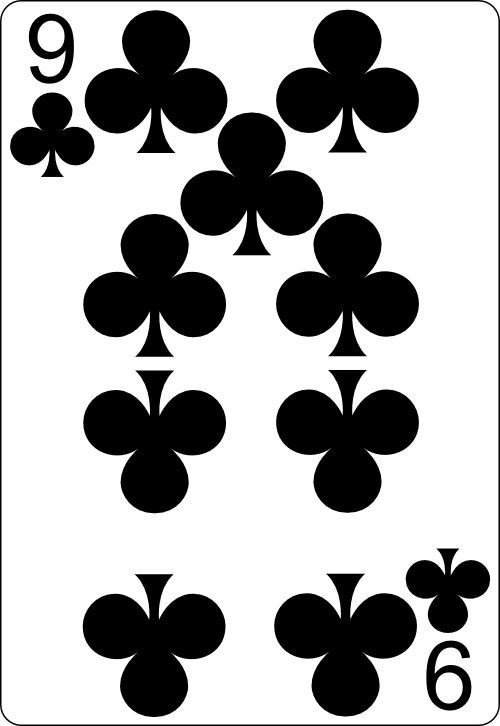
\includegraphics[height=\cardheight]{cards/9_of_clubs.png}}
\newcommand{\ninediamonds}{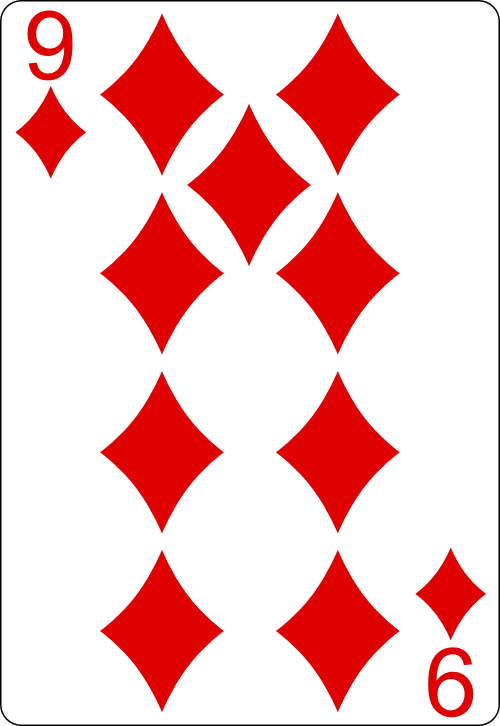
\includegraphics[height=\cardheight]{cards/9_of_diamonds.png}}
\newcommand{\ninehearts}{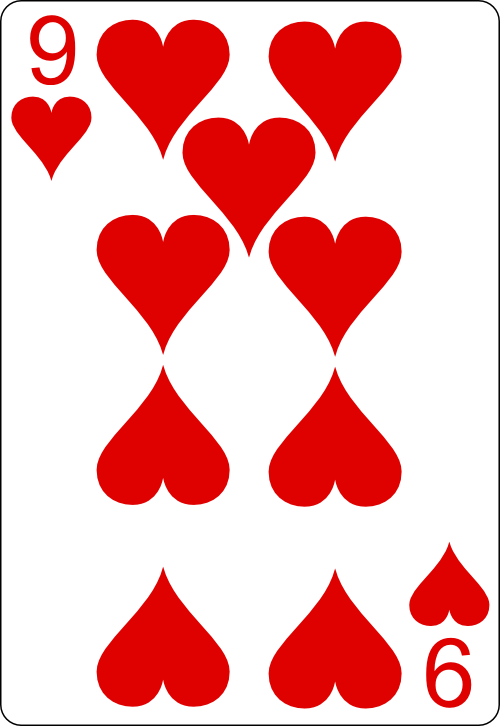
\includegraphics[height=\cardheight]{cards/9_of_hearts.png}}
\newcommand{\ninespades}{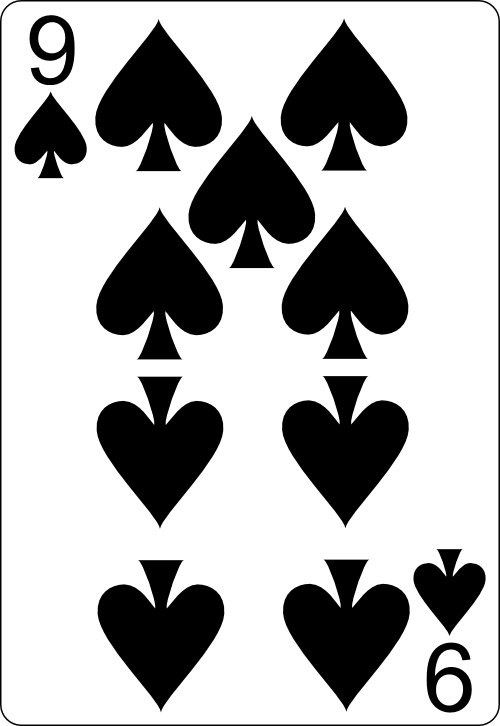
\includegraphics[height=\cardheight]{cards/9_of_spades.png}}
\newcommand{\aceclubs}{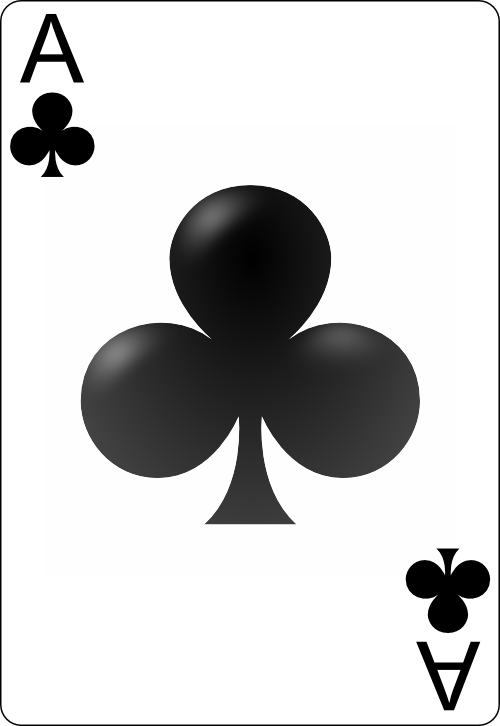
\includegraphics[height=\cardheight]{cards/ace_of_clubs.png}}
\newcommand{\acediamonds}{
\includegraphics[height=\cardheight]{cards/ace_of_diamonds.png}}
\newcommand{\acehearts}{
\includegraphics[height=\cardheight]{cards/ace_of_hearts.png}}
\newcommand{\acespades}{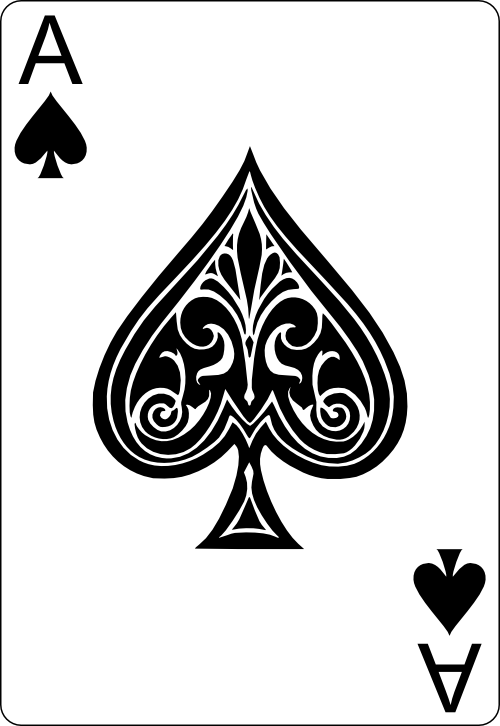
\includegraphics[height=\cardheight]{cards/ace_of_spades.png}}
\newcommand{\jackclubs}{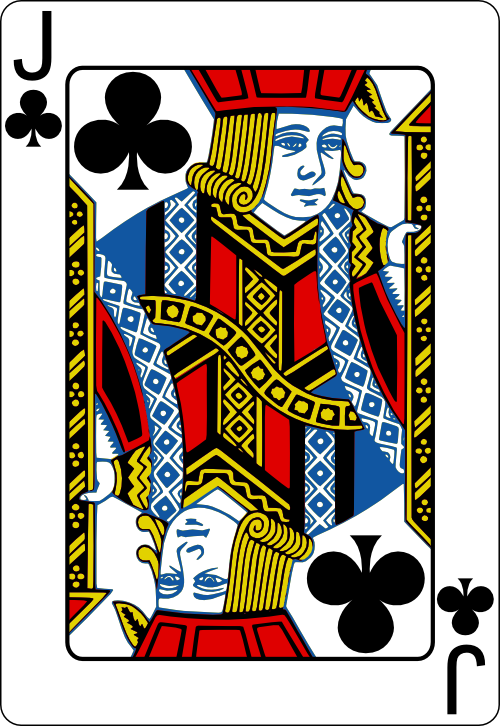
\includegraphics[height=\cardheight]{cards/jack_of_clubs.png}}
\newcommand{\jackdiamonds}{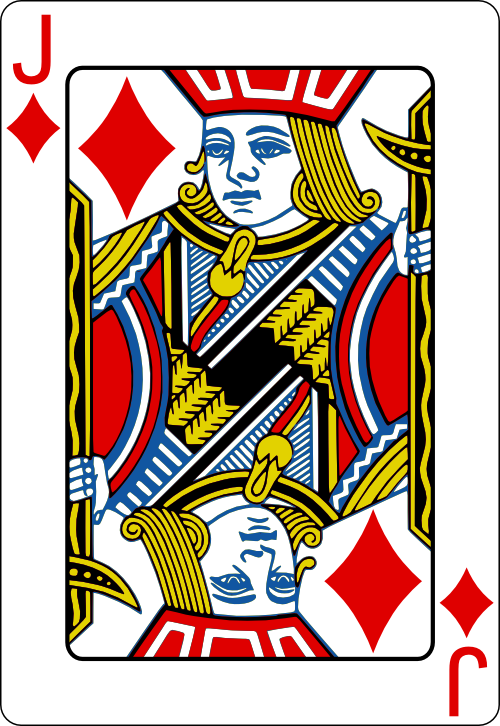
\includegraphics[height=\cardheight]{cards/jack_of_diamonds.png}}
\newcommand{\jackhearts}{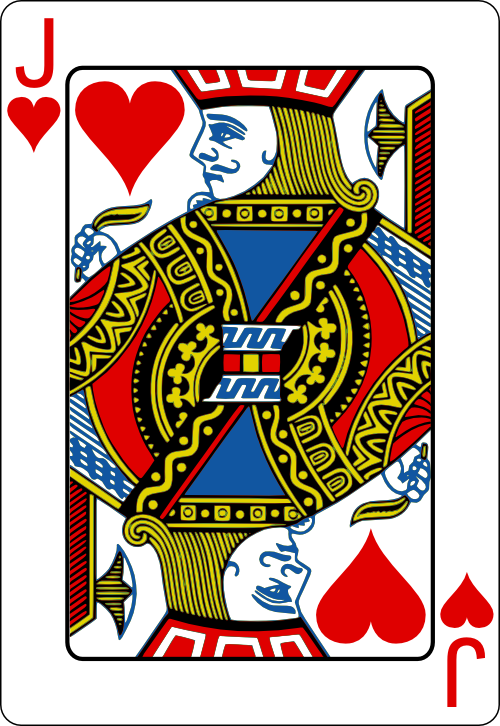
\includegraphics[height=\cardheight]{cards/jack_of_hearts.png}}
\newcommand{\jackspades}{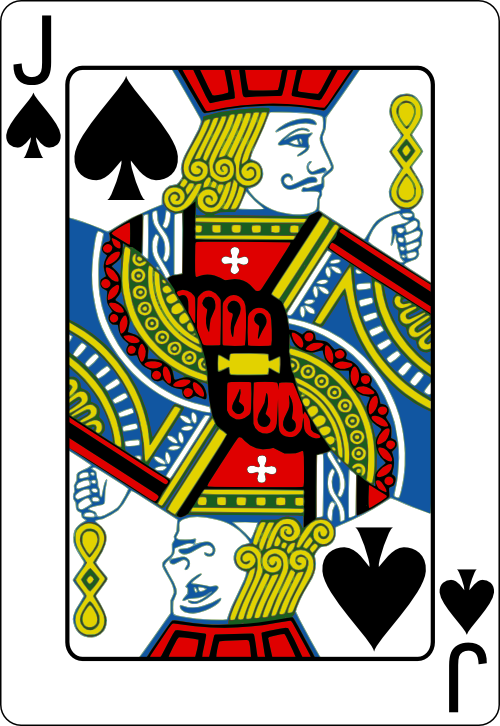
\includegraphics[height=\cardheight]{cards/jack_of_spades.png}}
\newcommand{\kingclubs}{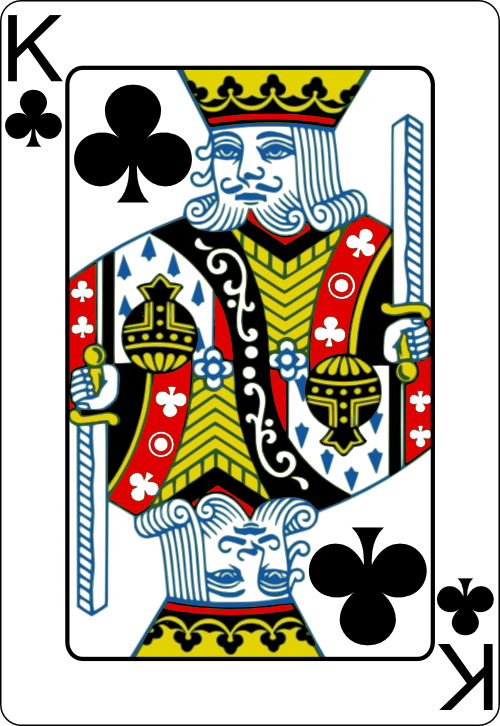
\includegraphics[height=\cardheight]{cards/king_of_clubs.png}}
\newcommand{\kingdiamonds}{
\includegraphics[height=\cardheight]{cards/king_of_diamonds.png}}
\newcommand{\kinghearts}{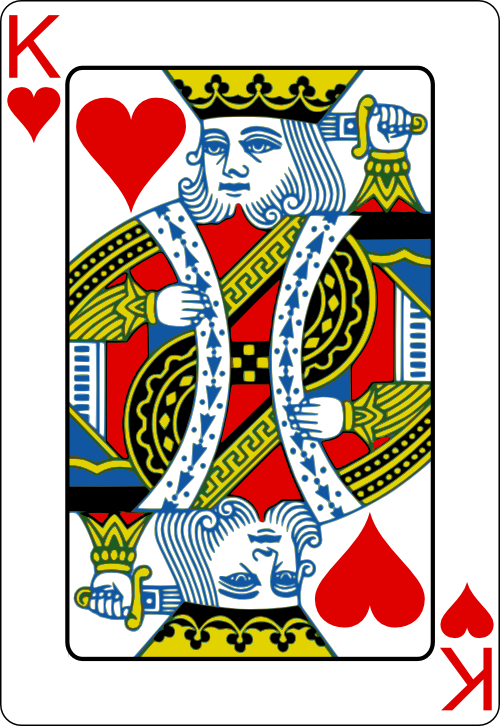
\includegraphics[height=\cardheight]{cards/king_of_hearts.png}}
\newcommand{\kingspades}{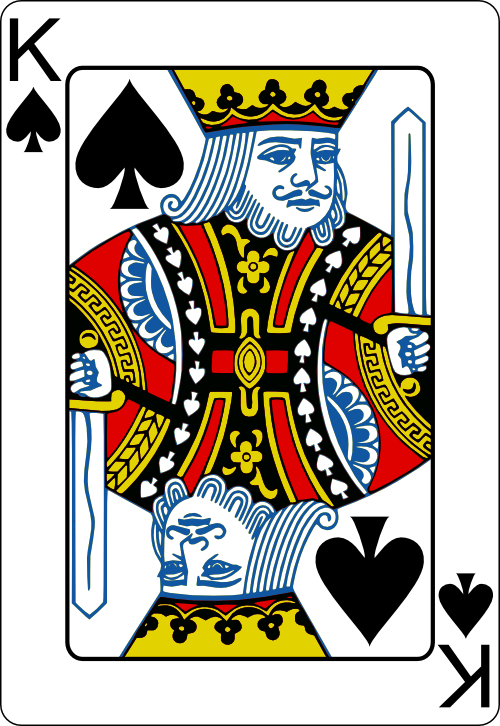
\includegraphics[height=\cardheight]{cards/king_of_spades.png}}
\newcommand{\queenclubs}{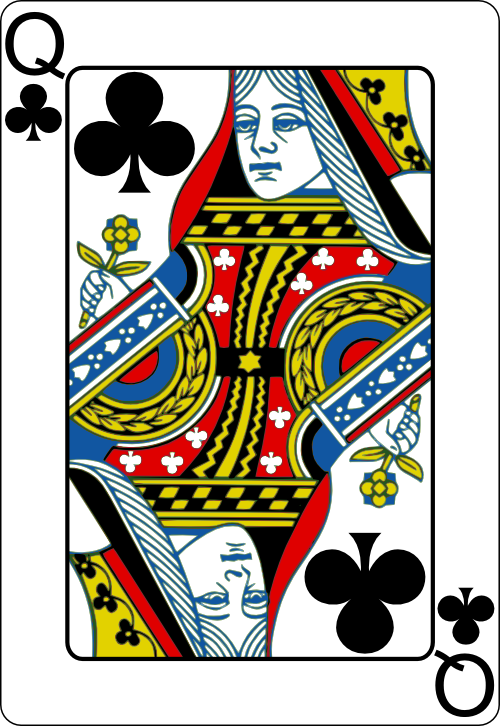
\includegraphics[height=\cardheight]{cards/queen_of_clubs.png}}
\newcommand{\queendiamonds}{
\includegraphics[height=\cardheight]{cards/queen_of_diamonds.png}}
\newcommand{\queenhearts}{\includegraphics[height=\cardheight]{cards/queen_of_hearts.png}}
\newcommand{\queenspades}{\includegraphics[height=\cardheight]{cards/queen_of_spades.png}}



\hspace{0pt}

\vfill

\begin{center}
	\includegraphics[scale=0.4]{uni_logo}
	
	\vspace{1cm}
	
	{\Large \textbf{Interim Report:} \pn \ Poker } \linebreak
	
	\begin{large}
		James Scully (4304469) \\
		psyjs20@nottingham.ac.uk \\
		G400 Computer Science \\
	\end{large}
	
\end{center}

\vfill

\begin{center}
	\textbf{Project Supervisor:} Milena Radenkovic
\end{center}

\hspace{0pt}

\pagebreak


\newcommand{\entry}[1]{
	\textbf{#1} - 
}

\newcommand{\TODO}[1]{
	\textbf{{\Large \emph{#1}}}
}



%%%
% Page 1: 
%%%

\section*{Introduction}




\section*{Motivation}
Rekop poker aims to provide an alternative to other multi-player applications on the Android app store as many of these prevent user customization and introduce in-app purchases, with no ability for players to play locally on their own network. 




\section*{Related Work}




\section*{Description}



\section*{Methodology}

Test-Driven Development has been essential so far in the development of the poker algorithm. Evaluating Texas Hold'em hands has many vectors of errors and being able to write tests before and alongside implementation helped out immensely. 

Take this snippet from the testing whether a hand is a straight or not: 

\begin{lstlisting}*[language=java]
assertTrue(new TexasEvaluator("0D 0D 2D KD AD QD JD").isStraight());
assertTrue(new TexasEvaluator("AD KD QD JD 0D QD JD").isStraight());
assertTrue(new TexasEvaluator("0D 2D 0D 9D 8D 7D 6D").isStraight());
assertTrue(new TexasEvaluator("2D 3D 4D 5D 6D QD JD").isStraight());
assertTrue(new TexasEvaluator("0D 0D 2D KD AD QD JD").isStraight());
assertTrue(new TexasEvaluator("KD QD JD JD JD 0D 9D").isStraight());
/* Falses */
assertFalse(new TexasEvaluator("0D 0D 0D 0D AD QD JD").isStraight());
assertFalse(new TexasEvaluator("2D 5D 9D JD 0D QD JD").isStraight());
assertFalse(new TexasEvaluator("kD 2D 0D 4D 8D 7D 6D").isStraight());
assertFalse(new TexasEvaluator("2D 3D 9D 3D 4D QD JD").isStraight());
\end{lstlisting}

Regarding the vectors of error, having instantenous feedback, whereby it was easy to debug providing breakpoints, the actual outcome and generally a sense of direction.










\section*{Design}

\subsection*{Algorithms}

\entry{Hand Strength}



\entry{Win evaluation}





\section*{Implementation}




\section*{Progress}
\subsection*{Management}

The first point of attack was to be the planning documents - enlisting our ideal creation and pseudocode simultaneously. However, upon writing pseudocode it became evident that there was much that would be looked over. 

It becomes very difficult to implement certain hands, such as a straight flush 


\subsection*{Contributions and Reflections}

\newpage
\TODO{Reflect - How hard evaluating a hand of poker can be; was not a simple process and underestimated. I.e. Talk about how detecting whether a straight may not be the most powerful, if a flush exists.}


A key goal of all software is that it must be efficient - both in terms of code complexity and performance. Upon undertaking this project it was naively assumed that, given how easy it is to recognize the outcome of a poker round in reality, it musn't be too difficult to implement efficiently through code. 

Evaluating poker hands efficiently becomes very complex and convoluted once the amount of hands possible is realised and how determining the outcome of some hands can be tricky. \\




Reflecting upon how I assumed Test-Driven Development would take much of our time before and during up and that we did not have "too much time to write tests and develop a fully-functional program", I couldn't have been further from the truth. Having instant feedback on whether it passed, what the result was and the ability to debug into it was essential. \\

Although, initially I was under the assumption that each test case was going to have to be made up of newly created objects. Frustrated that test cases were taking too long and a nuisance to write, I created a factory pattern within the evaluator class itself to resolve, for example, "0D 0D 2D KD AD QD JD" into an actual hand + table.  \\

I believe that the examples below really do speak for themselves. 

\begin{minipage}{.5\textwidth}

\begin{lstlisting}[
language=java,
basicstyle=\small
]
TexasHand FLUSH_FOK = new TexasHand(
    new Card(Suit.CLUBS, Face.FOUR),
    new Card(Suit.CLUBS, Face.FOUR),
    new Card(Suit.CLUBS, Face.FOUR),
    new Card(Suit.CLUBS, Face.FOUR),
    new Card(Suit.CLUBS, Face.ACE)
);
...
public void isFlush() {
    assertTrue(FLUSH_FOK.isFlush());
\end{lstlisting}
\end{minipage}

\textbf{New: } \\
assertTrue(new TexasEvaluator("AD KD JD QD 0D QS JC").isRoyalFlush());
); 







\section*{Bibliography}



\end{document}